\section{Literature Review}
\setlength{\parindent}{10ex}
In this review I cover the different approaches for predicting bathymetry.
The two main methods for collecting bathymetry data are \ac{SDB} and \ac{EGM}.
There is also a third approach discussed that improves upon the idea of a \ac{EGM}.
I also discuss echo sounders for precise measurements of bathymetry \cite{farr1980multibeam}.

\subsection{Machine Learning}
Machine Learning can be defined as the process of fitting a model to data with a algorithm \cite{bishop2006pattern}.
Predictions can then be produced from the models by supplying new data.
To validate the predictions, the supplied data's result is known.
For example, a model is trained to predict if a image contains a car.
Data from the images are extracted and used to train the model.
Images with cars can be considered positive images.
Images with out cars can be considered negative images.
New images that are labeled as positive or negative are given to the model for validation.
If the model successfully predicts the labels it will have a high accuracy and be a "valid" model.
The two main types of models in Machine Learning is classification and regression models.
There are several high level descriptions of classification and regression models including: supervised learning, unsupervised learning, and reinforcement learning.

\par
Classification models are models that predict a discrete value.
For example, the car model mentioned earlier.
The model predicts a discrete value of either positive or negative.
These types of models are effective at predicting values that can be grouped into "labeled" data.
Classification models can also be combined to form ensemble models.
A ensemble is a combination of "weaker" predictors to form a strong predictor.
%Include citations BELOW!!!!!
Examples of classification models used in this project include: Decision Trees, Naive Bayes, MLP Classifier, Quadratic Discriminant Analysis Classifier, and K Nearest Neighbors Classifier.
Examples of ensemble classifieres used in this project include: Random Forest Classifier, Ada boost, Gradient Boosting, Bagging, and Voting.

\par
Regression models predict a continous value.
For example, predicting water depth as a number is a continous value.
Where the range of predicted values is from sea level to the known depth of the ocean.
Essentially, this model represents a mathematical function where the input data is the function parameters.
This method is best when the desired result can not be grouped into discrete "labeled" data.

\par
Unsupervised learning describes a model that is trained without labels.
Meaning that the data does not have corresponding "ground-truth" values for predictions \cite{bishop2006pattern}.
Training a model without "ground-truth" is used for grouping similar values together programatically.
Ideal for identifying correlations in data that is otherwise unrelated and unlabeled.

\par
Supervised learning describes a model that is trained with labels \cite{bishop2006pattern}.
Training is guided or supervised by comparing results to labeled data.
This method of training is effective at fitting accurate models, and is used in this project for predicting bathymetry.
All models trained in this project use supervised learning.
Each model used will be discussed in subsequent sections.

\subsubsection{Bias and Variance}
%Describe the Bias and Variance relationship!
The generalized error of a model can be expressed in terms of bias and variance.
Bias is the average error of a model for different training sets.
Variance describes the sensitivity of the model to data.
These two terms are nessassary to understand the bias-variance problem.
This problem applies to all forms of supervised learning \cite{geman1992neural} and describes the indirect relationship of bias and variance.
The relationship being the minimization of bias often causing high variance, and minimizing variance often causing high bias.
Optimally, accuracte models should have a low bias and variance.

%Include image showing bias and variance here!!
\begin{figure}[h]
    \centering
    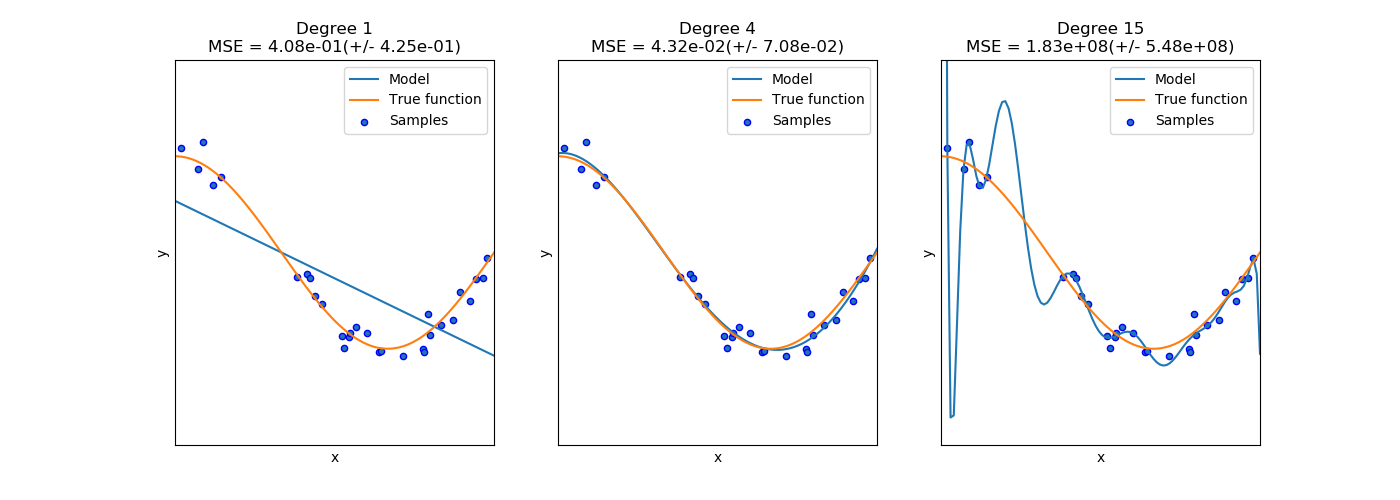
\includegraphics[scale=0.5]{sphx_glr_plot_underfitting_overfitting_001.png}
    \caption{Figure showing Bias and Variance examples}
    \label{}
\end{figure}

\subsubsection{Decision Trees}
%Talk about decision trees here
Decision trees are supervised models that are used for classification or regression \cite{breiman2017classification}.
They are simple to understand and interpret due to their simple decision structure. 
They are suseptable to over fiiting and can create overly complex trees that do not generalize well.
Over fitting is where a model will fit to closely to a training set \cite{cawley2010over}. 
Making it unable to make accurate predictions on data outside of what was used in training.

\begin{figure}[h]
    \centering
    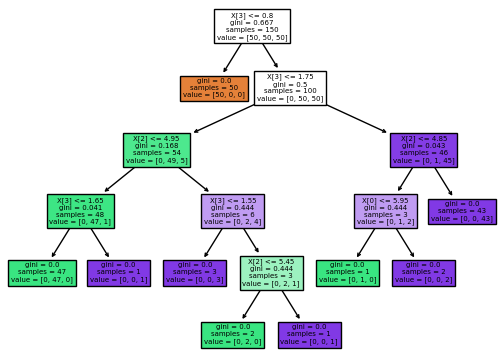
\includegraphics[scale=0.5]{dtreesepal.png}
    \caption{Figure showing example of Decision Tree}
    \label{}
\end{figure}

%Talk about random forest here
\par
The Random Forest Classifier is a ensemble of many decision trees \cite{breiman2001random}.
It fits a number of decision trees on various sub samples of the dataset.
This also helps to control over fitting because each tree is fit to a sub sample of the dataset.
It averages the prediction of each tree to make a more accurate prediction than any single tree.


\subsubsection{Boosting}
%Talk about Ada Boost here
Boosting describes a type of ensemble that is concerned with reducing bias.
The idea being to build base estimators sequentially and then use the results of each to train a different estimator with the intention of reducing bias.
Adaboost is an example of one such model \cite{freund1995desicion}.
Its core principle being the fitting of weak learners on many random samples of the training data.
This learners are then combined with a majority weighted vote. 
This process is iterated for the training phase.



%Talk about Gradient Boosting Here
%Need to finish this paragraph....
\par
The gradient boosting classifier is an ensemble of trees similar to a random forest classifier.
In gradient boosting, decision trees are used as "weak" learners.
They are gradually added to the model in order to reduce the error.
This "gradient decent" approach is effective at building a successful classifier.
These types of boosting algorithms tend to overfit the model.
This can be solved by enforcing tree constraints and random sampling of data.


\subsubsection{Averaging}
Averaging ensembles operate by aggregating the predictions of many models trained on random sub sets of the training data.
Introducing randomization into the training will often reduce the variance of the resulting ensemble.
Bagging is a example of a averaging ensemble and has several implementations.
The Bagging ensemble uses a single classifier and fits instances of it to random samples of the training data.
The predictions are then aggregated and averaged for a final prediction.

%Talk about voting here
The voting classifier works by using the predictions of a set of conceptually different predictors as votes.
The majority vote (hard voting) or averaged vote (soft voting) is selected as the prediction.
This classifier is good for combining equally performing models in order to balance out individual weaknesses.

\subsubsection{K Nearest Neighbors}
%Talk about KNN for classification
The K Nearest Neighbors algorithm is a non-parametric algorithm for classification and regression \cite{altman1992introduction}.
K Nearest Neighbors for classification stores the instances of the training data and associated labels.
Predictions are made by computing the distance of new instances to the training set.

\subsubsection{Multi Layer Perceptron}
%Talk about MLP Classifier here!!!
% Include MLP picture here I guess
The Multi Layer Perceptron is a model that fits a function iterativly through a process called back propogation.
The MLP classifier is a neural network model that is based on the structure of the human brain.
It consists of many layers beginning with an input layer.
The middle layers are called the "hidden layers" and are each assigned a weight.
Back propogation is used during training to adjust the weights in the hidden layers.
These adjustments are made to in order to reach a more accurate prediction.
There can be many hidden layers of differnt depths.
% Probably need to say more about the MLP Classifier...
% Maybe some graphics and other bull jive. Maybe a algorithm???

\begin{figure}[h]
    \centering
    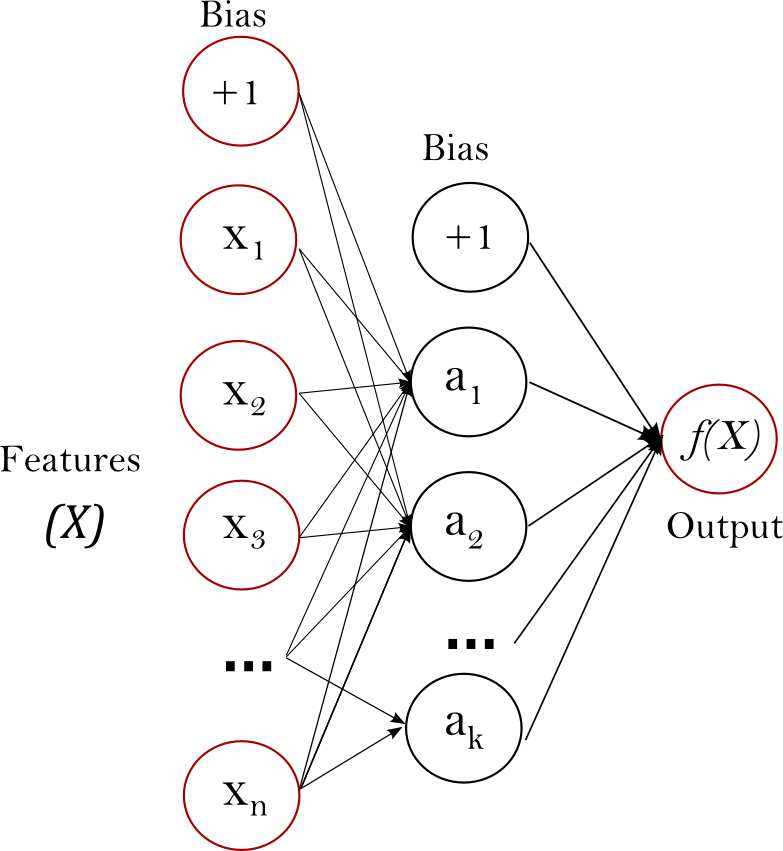
\includegraphics[scale=0.5]{multilayerperceptron_network.png}
    \caption{Figure showing Neural Network Model}
    \label{}
\end{figure}

%include more here about MLP


\subsubsection{Naive Bayes}
%Talk about Naive Bayes classifier here!!
The naive bayes classifier is based on applying the naive bayes theroem \cite{zhang2004optimality}.
The naive assumption of Naive Bayes is the conditional independence between pairs of features given the label.
Bayes theorem states the following relationship given class y and feature vector x.

% Put bayes theorem right here!!! Math mode I guess...


\subsubsection{Regression Models}
%Talk about Regression models used here...
Regression models are utilized for predicting continous values.
Specifically, regession is for approximating a function given a set of inputs to yield a output.
Linear regression is the simplest type and is concerned with fitting a linear combination of all training features.

% Put linear regression equation right here for the world to see YO

This project utilizes three regression models from sci kit.
The naive bayes\cite{sklearn_api}, logitic regression\cite{sklearn_api}, and svm regression\cite{sklearn_api} models are utlized for regression.

\subsection{Global Bathymetry Data}

\subsection{Echo Sounders (\ac{MBES})(\ac{SBES}) }
Echo sounders have been mounted on vessels for decades to accurately measure bathymetry.
The purpose of this is often for the ship to avoid running aground.
However, survey vessels have utilized \ac{MBES} systems to reliably create bathymetry charts \cite{farr1980multibeam}.
This can give a accurate measurement of bathymetry in all water depths.
This methods downside is the cost and time required to map global coverage.
A vessel must transport these sensors, and potentially take decades of expensive surveys to gain full global coverage.

%VERY VERY VERY IMPORTANT SECTION....2018 paper contains good content for my thesis!
\subsection{Satellite Derived Bathymetry (SDB)}
\ac{SDB} is a precise method of predicting coastal bathymetry. 
This method relies on the phenomena of light passing through a water column at a certain depth described by the Beer-Lambert law \cite{chybicki2018three}\cite{vinayaraj2016satellite}.
Sunlight passes through the water column and is reflected by the sediment at the bottom.
Satellites measure the attenuated light that is reflected from the bottom and uses the wavelength to estimate the depth of the column.
The technique accounts for atmospheric light absorption, water surface reflection, attenuation through and out of the column, and reflectance from the bottom sediment.
Clear waters are the best environment for this method which has the potential to predict bathymetry with a small RMSE \cite{chybicki2018three}.

\par
This method is important for its ability to predict swaths of bathymetry in shallow water.
Shallow waters where larger vessels can not sail, and large swaths of coastal waters are measured by \ac{SDB} in a cost and time effective processs.
For example, the marsh lands of Louisiana where water depth is only deep enough for flat bed vessels.
This method also has use in the scope of national defense for predicting or identifying changes in shallow water bathymetry.
These changes can be caused by sediments or man made objects. 

\par
The limitations of the \ac{SDB} method are based on water depth and clarity.
As depth increases light is unable to pass through the water column to the bottom.
The depth that light can penetrate is determined by the characteristics of the water.
Clear water will allow for much deeper depths to be predicted, where as murky, cluttered water limits the maximum depth.
Environmental characteristics such as sediment composition and weather affect the clarity of water \cite{vinayaraj2016satellite}.

\par
Current \ac{SDB} models can predict bathymetry with a \ac{RMSE} of less that 2.5 meters at a maximum depth of 50 meters.
Work performed by \cite{vinayaraj2016satellite} has improved the depth by using blue light sensing techniques.
Work performed by \cite{chybicki2018three} improved the accuracy by using advanced regression models when measuring the wavelengths.
\ac{SDB} models are ideal for coastal areas with a high water visibility.

\subsection{Aggregated Earth Gravitational Models (EGM)}
Work performed by Smith and Sandwell \cite{smith1994bathymetric}\cite{smith1997global} pioneered the use of Earth Gravitational Models (EGM).
They proposed that the relationship between seafloor topography and sea surface gravity is conveniently related \cite{smith1994bathymetric}.
Their work identified the wavelength bands at which this relation holds true.
They identified the areas that could be predicted with this relationship and used sparse ship soundings to fill in gaps of their predictions.
Areas with large seamounts found the correlation to be strongest, while areas of flat sediments found the correlation to be weakest.
They named this technique the "Inverse Nettleton Procedure" and used a simple linear regression model to exploit this correlation and improve existing aggregated datasets.

\begin{equation}
    b(x) = D(x) + s(x)g(x)
\end{equation}

\par
Smith and Sandwell aggregated their predicted values from their \ac{EGM} with ship based Multi Beam Echo Sounding sonar data.
The sonar data is sparse, but provides accurate readings of the ocean's bathymetry.
This aggregation yielded global coverage up to 81 degrees.
The aggregation yielded prediction accuracy within ~100 meters in coastal waters, and ~200 meters in the global ocean space.

%Discuss the STRM Global Dataset here in detail....
\par 
This work was later improved in \cite{becker2009global}.
The model was substantially improved by increasing the number of ship soundings and increasing the aggregation sources.
Ten external datasets were aggregated for the SRTM30 grid.
Agencies in these sources include \ac{NAVO}, \ac{GEBCO}, \ac{NOAA}, \ac{NGA}, and \ac{JAMSTEC}.
These datasets include high resolution coastal bathymetry from around the world and greatly increased the global accuracy.

%Spelling check big time bruh
\par
The limitations of aggregated \ac{EGM}s is based on correlation uncertainty and unknown ocean features.
Sediment density drives the correlation between sea surface gravity and bathymetry.
A dense geoid will generate greater sea surface gravity than a less dense geoid.
Flat sea floors with a less dense composition can appear lower than normal.
This is all controlled by the scaling factor described in \cite{smith1994bathymetric} and shown in equation 1. 
However, there is not a optimal scaling factor for the entire world.
Identifying an optimal scaling factor for an area will require knowledge of the sediment type in the global scale.


\subsection{Machine Learning Optimized \ac{EGM}}
The aggregated \ac{EGM} is a physics based model that wants the relationship between gravity and bathymetry to be directly correlated.
This correlation is often non-trivial to define due to environmental factors.
The nondeterministic behavior is compensated by the scaling factor mentioned in the previous section.
Attempts to optimize this scaling factor have been made, and \ac{ML} has shown much promise in this regard.

\par
The work preformed by \cite{jena2012prediction} used \ac{ML} to optimize their gravitational regression models.
Instead of identifying an optimal scaling factor deterministically, they used an \ac{ANN} to optimize the scaling factor.
This was done using precise \ac{MBES} data as truth data and satellite altimeter data.
This method was tested on a localized swatch of ocean in the Arabian Sea.

\par
This optimization improved upon the current physics models.
Their model could predict bathymetry within a \ac{RMSE} of ~129 meters for flat sea floor.
Geoids resulted in a \ac{RMSE} of ~179 meters.
Both of these results are globally similar with aggregated models, while boasting increased accuracy in their localized training area of the Arabian Sea.

%\subsection{Machine Learning Models}